%!TEX TS-program = xelatex

% Официальный шаблон презентации НИУ ВШЭ в beamer (LaTeX)
% Версия 2.0
% Язык — русский

\documentclass[aspectratio=169]{beamer}

\newbool{russian}
\booltrue{russian}
\usepackage{HSE-theme/beamerthemeHSE}

%%% Работа с русским языком и шрифтами
\usepackage{multirow}
\usepackage{listings} 
\usepackage[dvipsnames]{xcolor}
\usepackage[english,russian]{babel}
\usepackage[no-math]{fontspec}
\usepackage{makecell}
	\IfFontExistsTF{HSE Sans}
		{\newcommand{\presentationfont}{HSE Sans}}
		{\newcommand{\presentationfont}{Arial}}
	\setsansfont{\presentationfont}
	\setmonofont{Courier New}

\usepackage{mathspec}
	\setmathsfont(Digits,Latin,Greek)[Numbers={Lining,Proportional}]{\presentationfont}
	\setmathrm[Numbers={Lining,Proportional}]{\presentationfont}
\uselanguage{russian}
\languagepath{russian}
\deftranslation[to=russian]{Theorem}{Теорема}
\deftranslation[to=russian]{Definition}{Определение}
\deftranslation[to=russian]{Definitions}{Определения}
\deftranslation[to=russian]{Corollary}{Следствие}
\deftranslation[to=russian]{Fact}{Факт}
\deftranslation[to=russian]{Example}{Пример}
\deftranslation[to=russian]{Examples}{Примеры}

\usepackage{booktabs}
\usepackage{array}
\graphicspath{{images/}}


\newcommand{\term}[1]{{\large\textcolor{HSEblue}{#1}}}
\newcommand{\cmd}[1]{\textcolor{HSEblue}{\texttt{#1}}}
\newcommand{\todo}[1]{\textcolor{red}{[TODO: #1]}}

\newenvironment{demoblock}[1]
	{\begin{exampleblock}{Демо: #1}\small}
	{\end{exampleblock}}

\lstset{ 
    basicstyle=\color{HSEblue}\ttfamily\small,
    numbers=left,
    numberstyle=\color{HSEblue}\ttfamily\scriptsize,
    frame=single,
    columns=fullflexible,
    keepspaces=true,
    showstringspaces=false,
    breaklines=true,
    rulecolor=\color{HSEblue},
}


%% Информация об авторе и выступлении

\title[Мобильные колесные роботы]{Симуляторы в робототехнике. Знакомство с Webots}
\subtitle{Проектный семинар <<Мобильные колесные роботы>>}
\author[Команда курса]{Дергачев Степан  Алексеевич, \texttt{\href{mailto:sadergachev@hse.ru}{sadergachev@hse.ru}} \\ Муравьев Кирилл Федорович, \texttt{\href{mailto:kmuravev@hse.ru}{kmuravev@hse.ru}}}
\institute{Факультет компьютерных наук НИУ ВШЭ}
\date{24 сентября 2026}

\begin{document}


\frame[plain]{\titlepage}

\section{Основы симуляции}

\begin{frame}
\frametitle{Симуляторы в робототехнике}
\begin{block}{Основные плюсы}
\begin{itemize}
  \small
  \item Разработка и проверка алгоритмов, если реальные роботы недоступны
  \item Проверка безопасности алгоритмов без поломки оборудования
  \item Повторение одного сценария для сравнения алгоритмов, проведение массовых экспериментов
  \item Сбор данных для алгоритмов, основанных на обучении, массовые запуски при онлайн-обучении
  \item Доступ к истинному состоянию для проведения экспериментов и точной оценки алгоритмов, регулирование шума входных данных
  \item Снижение сложности проведения экспериментов в целом, в частности при обучении робототехнике
\end{itemize}
\end{block}
\vfill
\begin{block}{Ограничение}
\small
Перенос алгоритмов на реального робота требует дополнительной проверки и настройки ({\color{HSEblue}sim2real gap}).
\end{block}
\end{frame}

\begin{frame}
\frametitle{Симуляторы в робототехнике}
\renewcommand{\arraystretch}{1.2}
\begin{tabular}{>{\raggedright\arraybackslash}m{0.30\textwidth}>{\raggedright\arraybackslash}m{0.68\textwidth}}
\toprule
\term{Что моделируется?} & \term{Примеры} \\
\midrule
Среда и сценарий & Объекты в среде, освещение, начальные условия. \\
Кинематика & Перемещение робота (и его частей) без учета сил.  \\
Динамика & Масса, инерция, силы, моменты. \\
Контакты & Столкновения тел, опора на пол, трение колёс. \\
Датчики и приводы & Рендеринг изображения камер, лучи LiDAR, энкодеры, управление моторами. \\
\bottomrule
\end{tabular}
\vfill
Детализацию выбирают под задачу: для поиска пути и для захвата предмета нужны модели разной точности.
\end{frame}

\begin{frame}
\frametitle{Базовый цикл симуляции}
\begin{enumerate}
  \item Получить доступные управляющие воздействия: моменты/угловые скорости моторов или другие воздействия от контроллеров 
  \item Рассчитать следующий шаг: применить правила движения, рассчитать силы, контакты и ограничения объектов мира
  \item Обновить состояние и время: сохранить новые положения и другие переменные состояния, увеличить время на $\Delta t$
  \item Отрисовать результаты: обновить виртуальные датчики и сформировать изображение.
\end{enumerate}
\end{frame}

\begin{frame}
\frametitle{Базовый цикл симуляции}
\begin{columns}[T]
\column{0.45\textwidth}
\begin{block}{Симуляционное время}
\begin{itemize}
  \item Изменяется дискретными шагами $\Delta t$.
  \item Может идти быстрее или медленнее реального времени.
  \item На паузе состояние мира не обновляется.
\end{itemize}
\end{block}
\column{0.49\textwidth}
\begin{block}{Точность}
\begin{itemize}
  \item Малый шаг $\Delta t$ увеличивает объём вычислений.
  \item Большой шаг может ухудшить устойчивость расчетов физики/контактов.
  \item Частоты физики, датчиков и отрисовки могут различаться.
\end{itemize}
\end{block}
\end{columns}
\end{frame}

\section{Обзор симуляторов}

\begin{frame}
\frametitle{Примеры симуляторов: простые 2D-среды}
  \begin{itemize}
    \item Не используют сложные физические расчеты/реалистичную графику/сложные модели датчиков 
    \item Удобны для простых и массовых экспериментов
    \item Редко обладают ROS интерфейсом
  \end{itemize}
\vfill
\renewcommand{\arraystretch}{1.1}
\small
\begin{tabular}{>{\raggedright\arraybackslash}m{0.16\textwidth}>{\raggedright\arraybackslash}m{0.74\textwidth}}
\toprule
\textcolor{HSEblue}{Пример} & \textcolor{HSEblue}{Основное направление} \\
\midrule
IR-SIM & Навигация агента/робота на плоскости, различные модели движения роботов, препятствия и датчики \\
POGEMA & Движение нескольких агентов по клеткам, совместный поиск путей (MAPF), обучение многоагентного RL \\
CAMAR & Движение нескольких агентов в непрерывном пространстве, различные модели движения, обучение многоагентного RL \\
\bottomrule
\end{tabular}
\end{frame}

\begin{frame}
\frametitle{Примеры симуляторов: Gazebo}
\begin{columns}[T]
\column{0.55\textwidth}
\footnotesize
\begin{itemize}
  \item Стандартный многоцелевой симулятор, входящий в экосистему ROS.
  \item Моделирование физики, различных датчиков и типов роботов
  \item Использует форматы файлов, широко распространенные в ROS сообществе.
  \item Упрощенная визуальная составляющая, для получения более детальной картинки требуется долгая настройка
  \item Фактически привязан к платформе Linux и ROS (хотя работа без ROS допускается)
  \item  Разделен на два поколения: Classic и Ignition/Sim. Ignition находится в активной разработке, может быть нестабильным, отсутствуют часть функций и неактуальная документация

\end{itemize}
\column{0.44\textwidth}
  \vspace{30pt}
	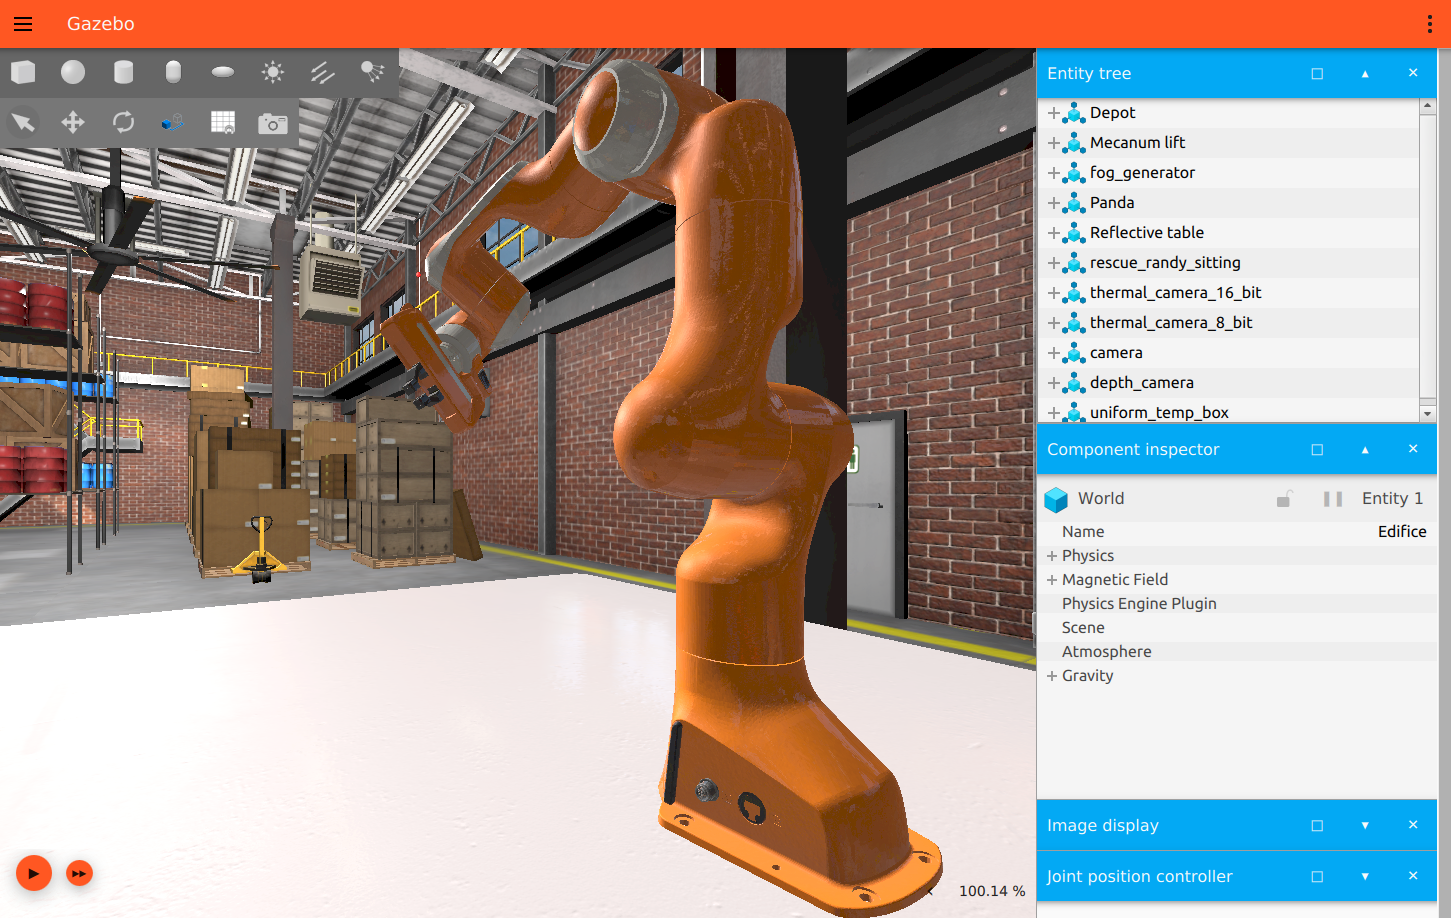
\includegraphics[width=0.99\columnwidth]{images/gazebo.png}
\end{columns}
\end{frame}

\begin{frame}
\frametitle{Примеры симуляторов: NVIDIA Isaac}
\begin{columns}[T]
\column{0.55\textwidth}
\small
\begin{itemize}
  \item Многоцелевой симулятор, построен на основе NVIDIA PhysX, обладает реалистичной визуализацией, включая RTX освещение.
  \item Включает большое количество инструментов для обучения и апробации методов на основе обучения, в том числе RL.
  \item Есть собственный API и интеграция с ROS. Однако имеет высокий порог входа. 
  \item Требуется производительный компьютер с NVIDIA GPU последних поколений и большим объемом видеопамяти.
\end{itemize}
\column{0.44\textwidth}
  \vspace{20pt}
	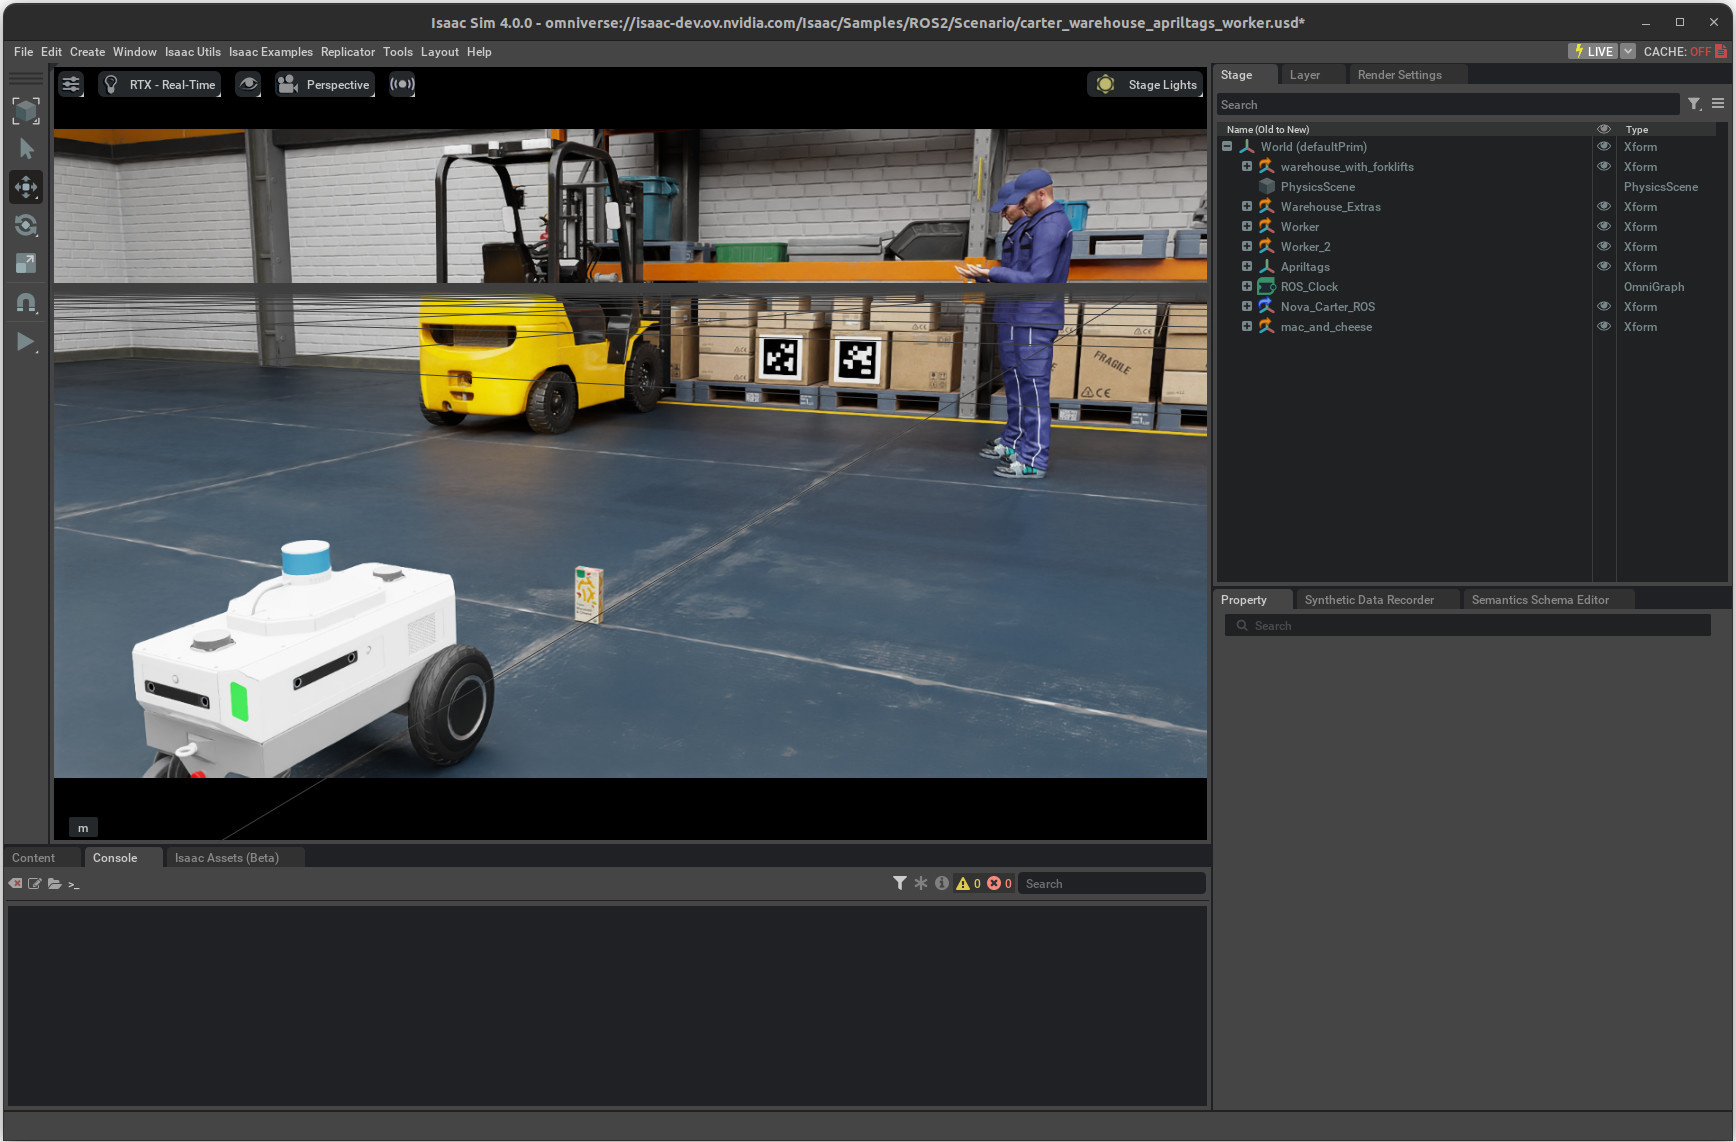
\includegraphics[width=0.99\columnwidth]{images/isaac.png}
\end{columns}
\end{frame}

\begin{frame}
\frametitle{Примеры симуляторов: MuJoCo}
\begin{columns}[T]
\column{0.55\textwidth}
\small
\begin{itemize}
  \item Симулятор, построенный на физическом движке для точного моделирования сложных систем из твёрдых тел, сочленений и контактов.
  \item Предоставляет API для управления симуляцией и роботом напрямую, существует интерфейс с ROS2
  \item Часто применяется для задач оптимального управления и обучения с подкреплением. В частности, для задач манипуляции
  \item Готовую робототехническую инфраструктуру обычно собирают и проверяют отдельно.
\end{itemize}
\column{0.39\textwidth}
	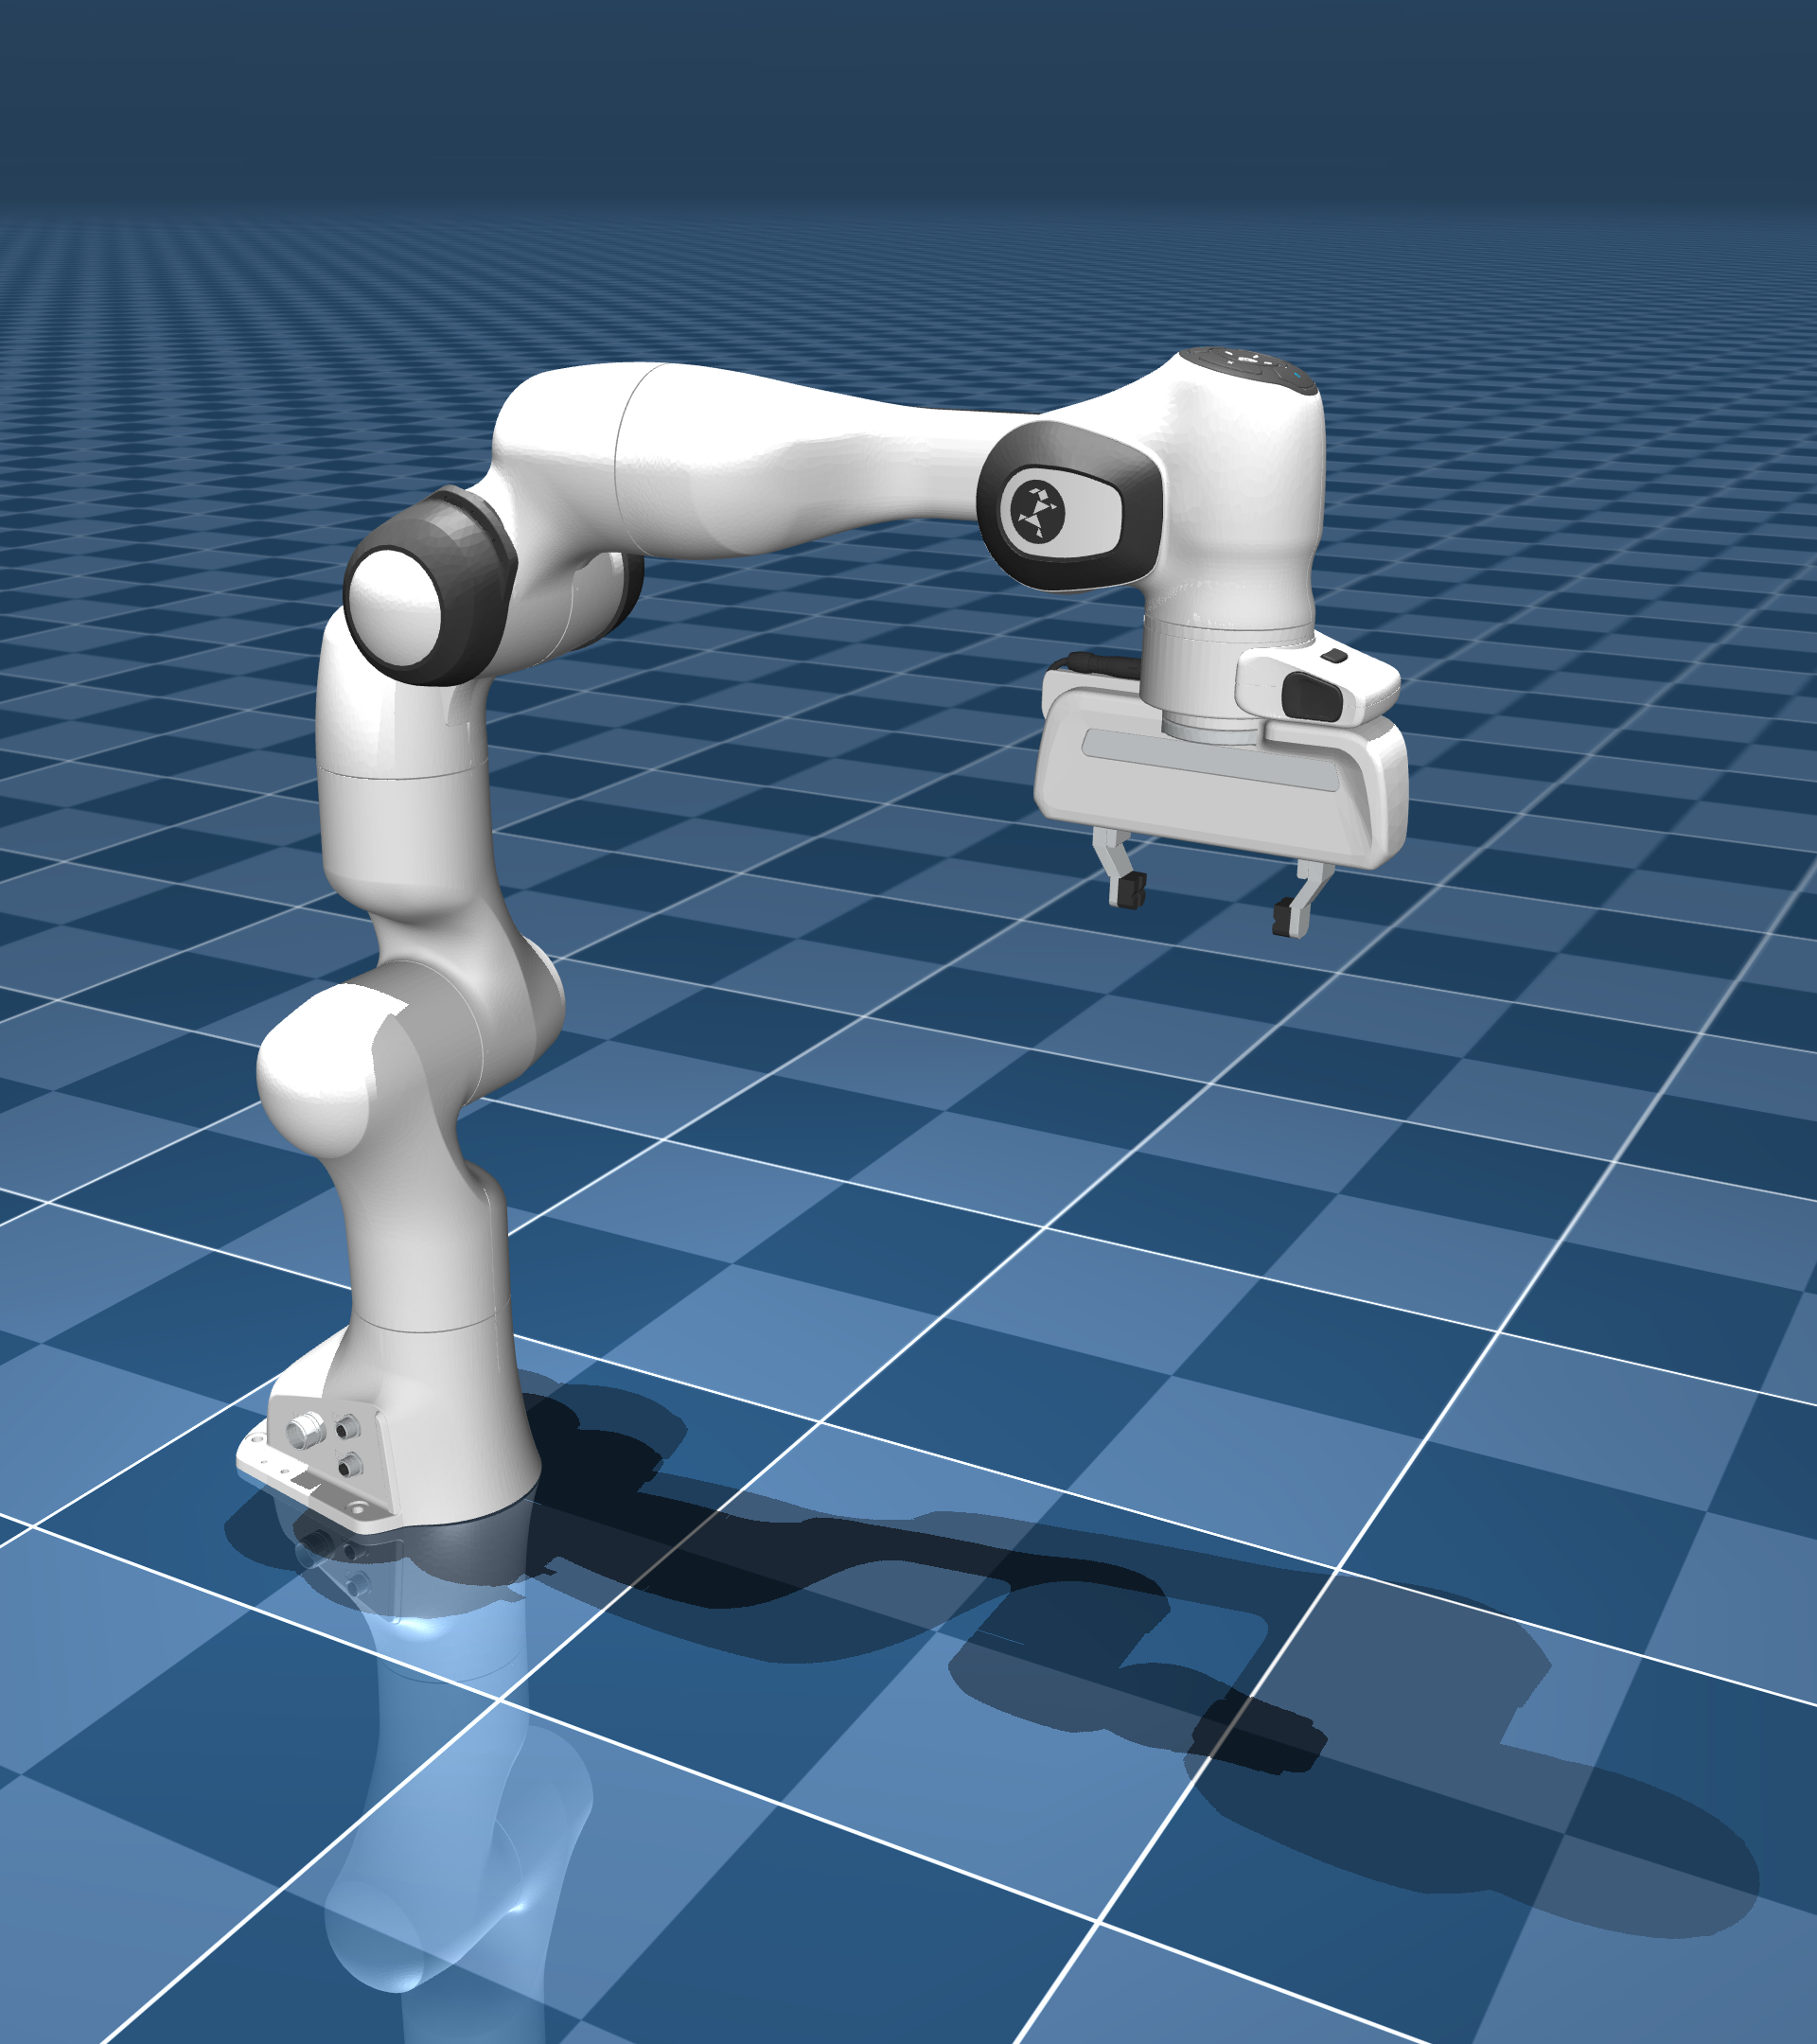
\includegraphics[width=0.99\columnwidth]{images/mujoco.png}
\end{columns}
\end{frame}

\begin{frame}
\frametitle{Примеры симуляторов: CARLA}
\begin{columns}[T]
\column{0.55\textwidth}
\small
\begin{itemize}
  \item Специализированная среда для исследований автономного вождения. Содержит моделирование автомобилей (с датчиками) и пешеходов, карты городов и управление транспортными потоками.
  \item Построена на основе Unreal Engine.
  \item Предоставляет API для управления симуляцией и автомобилями напрямую, существует интерфейс с ROS2
\end{itemize}
\column{0.44\textwidth}
  \vspace{10pt}
	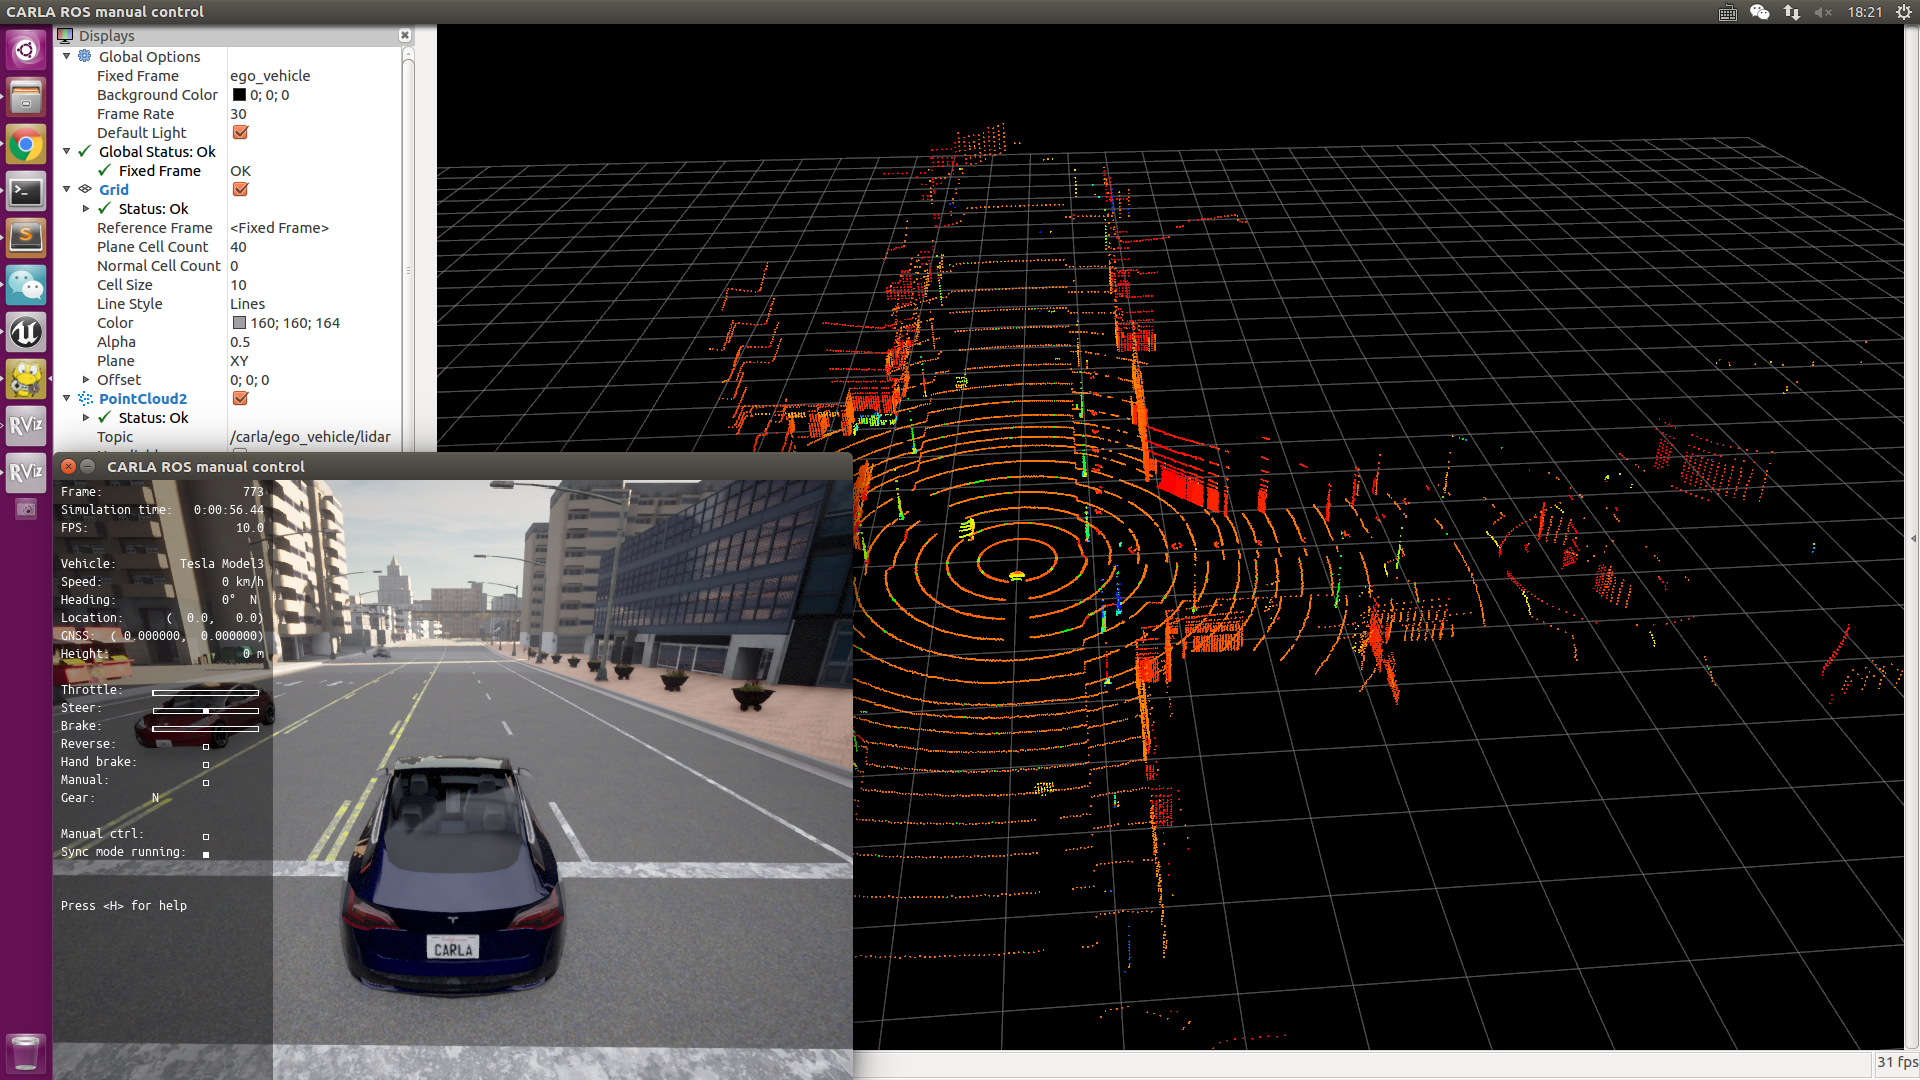
\includegraphics[width=0.99\columnwidth]{images/carla.png}
\end{columns}
\end{frame}

\begin{frame}
\frametitle{Примеры симуляторов: Webots}
\begin{columns}[T]
\column{0.55\textwidth}
\small
\begin{itemize}
  \item Многоцелевой симулятор, включает в себя моделирование физики, различных датчиков и типов роботов, современную и реалистичную визуализацию
  \item Обладает собственным API и интерфейсом к ROS2, но использует собственные форматы файлов, что немного затрудняет использование с ROS
  \item Обладает (в среднем) низким порогом входа для обучения и хорошей документацией
  \item Поддерживает различные платформы: Linux, Windows и macOS.
\end{itemize}
\column{0.44\textwidth}
  \vspace{30pt}
	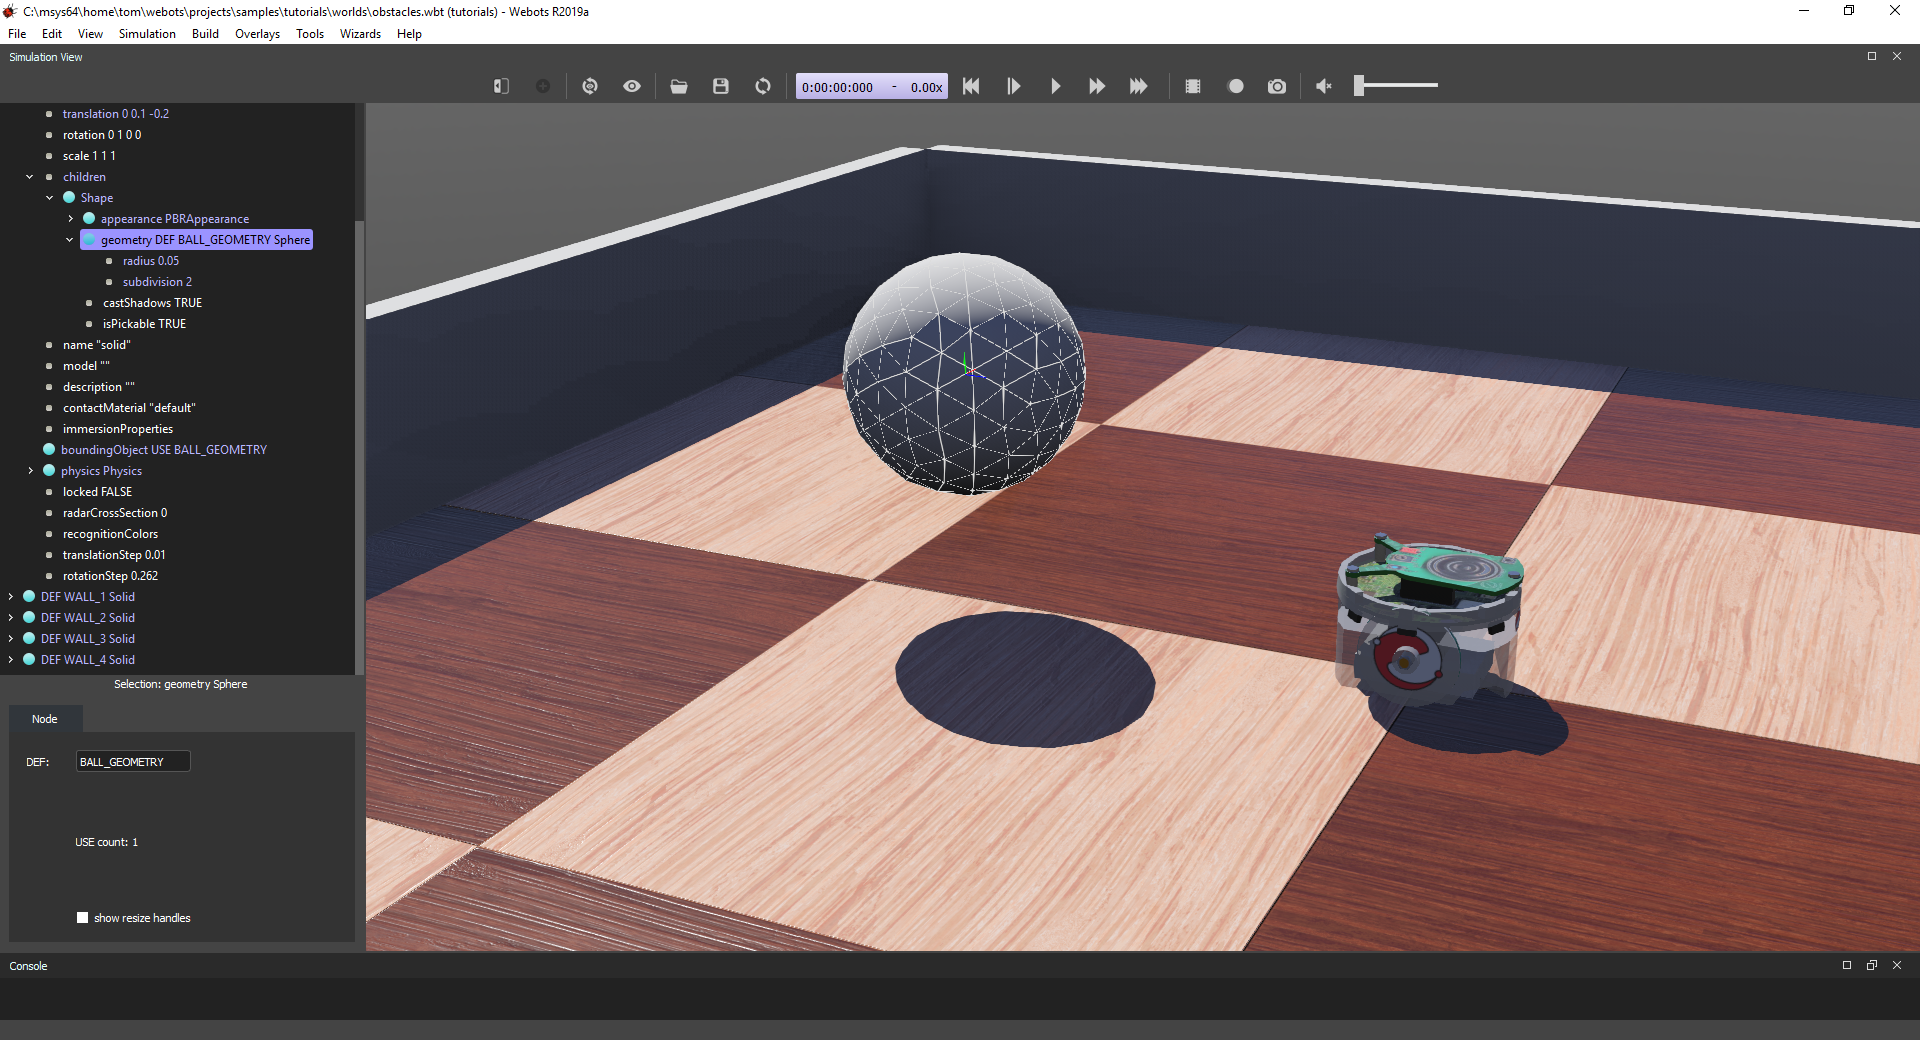
\includegraphics[width=0.99\columnwidth]{images/webots.png}
\end{columns}
\end{frame}



\section{Устройство Webots}

\begin{frame}
\frametitle{Устройство Webots}
\begin{columns}[T]
\column{0.46\textwidth}
\begin{block}{Сцена}
\begin{itemize}
  \item Сцена -- дерево, состоящая из узлов
  \item Описывается файлом \cmd{.wbt}, используется читаемый формат на основе VRML97
  \item Включает общие параметры симуляции, настройки точки наблюдения, описание объектов и роботов в сцене 
\end{itemize}
\end{block}
\column{0.50\textwidth}
\begin{block}{Узел}
\begin{itemize}
  \item Узел -- базовая единица-объект в сцене.
  \item Узел имеет тип и поля
  \item Поля задают значения или вложенные узлы.
  \item Вложенность задаёт структуру и локальные системы координат.
  \item Шаблон переиспользуемых настраиваемых узлов можно сохранить в файле PROTO.
\end{itemize}
\end{block}
\end{columns}
\end{frame}

\begin{frame}
\frametitle{Строение узла}
\begin{columns}[c]
\column{0.49\textwidth}
\begin{itemize}
  \item Базовый узел \cmd{Solid}
  \item \cmd{physics} -- параметры моделирования физики объекта (масса, плотность, материал и т.д.) 
  \item \cmd{boundingObject} -- модель расчета коллизий и контактов
  \item \cmd{children} -- дочерние объекты и/или описание видимой модели узла
\end{itemize}
\column{0.49\textwidth}
\centering
	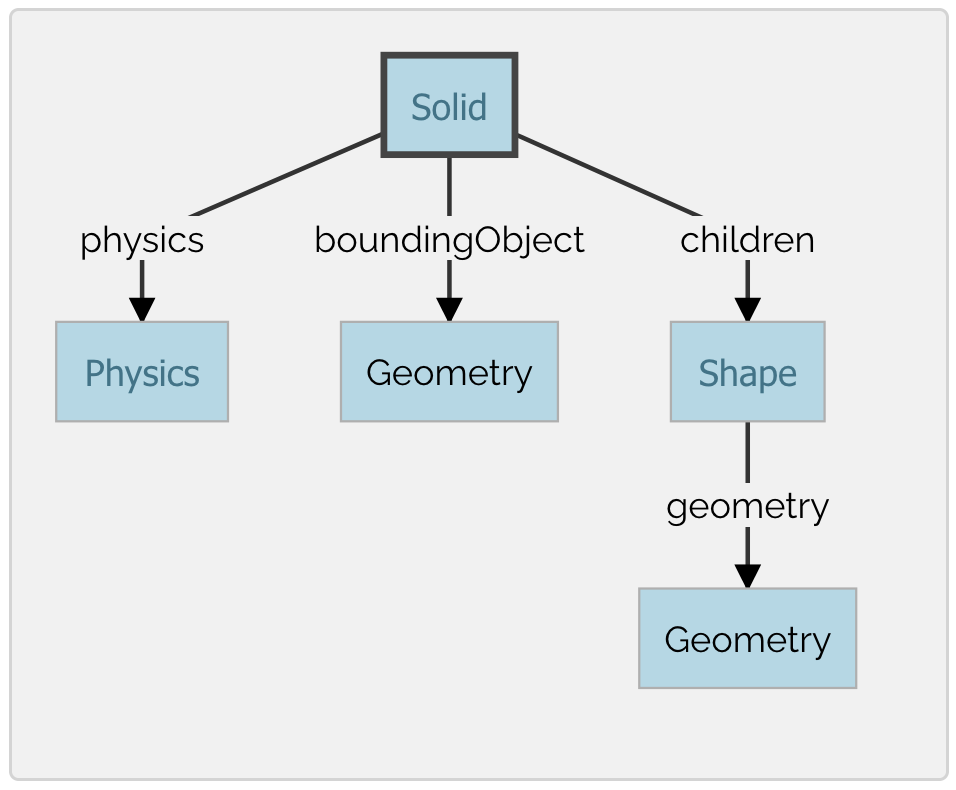
\includegraphics[height=0.8\textheight]{images/node.png}
\end{columns}
\end{frame}

\begin{frame}[fragile]
\frametitle{Пример простого объекта}
\begin{columns}[T]
\column{0.5\textwidth}
\begin{lstlisting}[basicstyle=\color{HSEblue}\ttfamily\footnotesize]
Solid {
  translation 1 0 0.2
  children [
    Shape {
      geometry DEF BOX Box {
        size 0.1 0.1 0.1
      }
    }
  ]
  boundingObject USE BOX
  physics Physics {
    density -1
    mass 1
  }
}
\end{lstlisting}
\column{0.43\textwidth}
\begin{itemize}
  \item Куб со стороной 0.1~м и массой 1~кг.
  \item Механизм \cmd{DEF}/\cmd{USE} позволяет повторно использовать геометрию.
  \item Если убрать \cmd{Physics}, то тело не будет двигаться под действием сил
  \item Без \cmd{boundingObject} не будут определяться контакты и столкновения. Поле \cmd{physics} тоже должно быть \cmd{NULL}.
\end{itemize}
\end{columns}
\end{frame}

\begin{frame}[fragile]
\frametitle{Пример PROTO}
\begin{columns}[T]
\column{0.50\textwidth}
\begin{lstlisting}[basicstyle=\color{HSEblue}\ttfamily\footnotesize]
PROTO CourseBox [
  field SFVec3f translation 0 0 0.2
  field SFVec3f size 0.4 0.4 0.4
  field SFFloat mass 1
]
{
  Solid {
    translation IS translation
    # ...
  }
}
\end{lstlisting}
\column{0.43\textwidth}
\begin{itemize}
  \item В PROTO узлу задаются доступные параметры (поля).
  \item \cmd{IS} связывает значение параметра с полем узла.
  \item \cmd{EXTERNPROTO} подключает шаблон из файла.
  \item Экземпляры могут отличаться параметрами.
\end{itemize}
\end{columns}
\vfill
\begin{lstlisting}[numbers=none,basicstyle=\color{HSEblue}\ttfamily\footnotesize]
#VRML_SIM R2025a utf8
EXTERNPROTO "../protos/CourseBox.proto"
CourseBox { translation 1 0 0.2  mass 2 }
\end{lstlisting}
\end{frame}

\begin{frame}
\frametitle{Описание робота}
\begin{columns}[c]
\column{0.49\textwidth}
\begin{itemize}
  \small
  \item Робот задается узлом типа \cmd{Robot}, который расширяет \cmd{Solid}
  \item У робота есть тело с геометрией и физикой, а также устройства и контроллер.
  \item \cmd{HingeJoint} + \cmd{RotationalMotor} + \cmd{PositionSensor} моделируют колесо с энкодером
  \item \cmd{Lidar}, \cmd{Camera}, \cmd{GPS}, \cmd{InertialUnit} моделируют датчики.
\end{itemize}
\column{0.49\textwidth}
	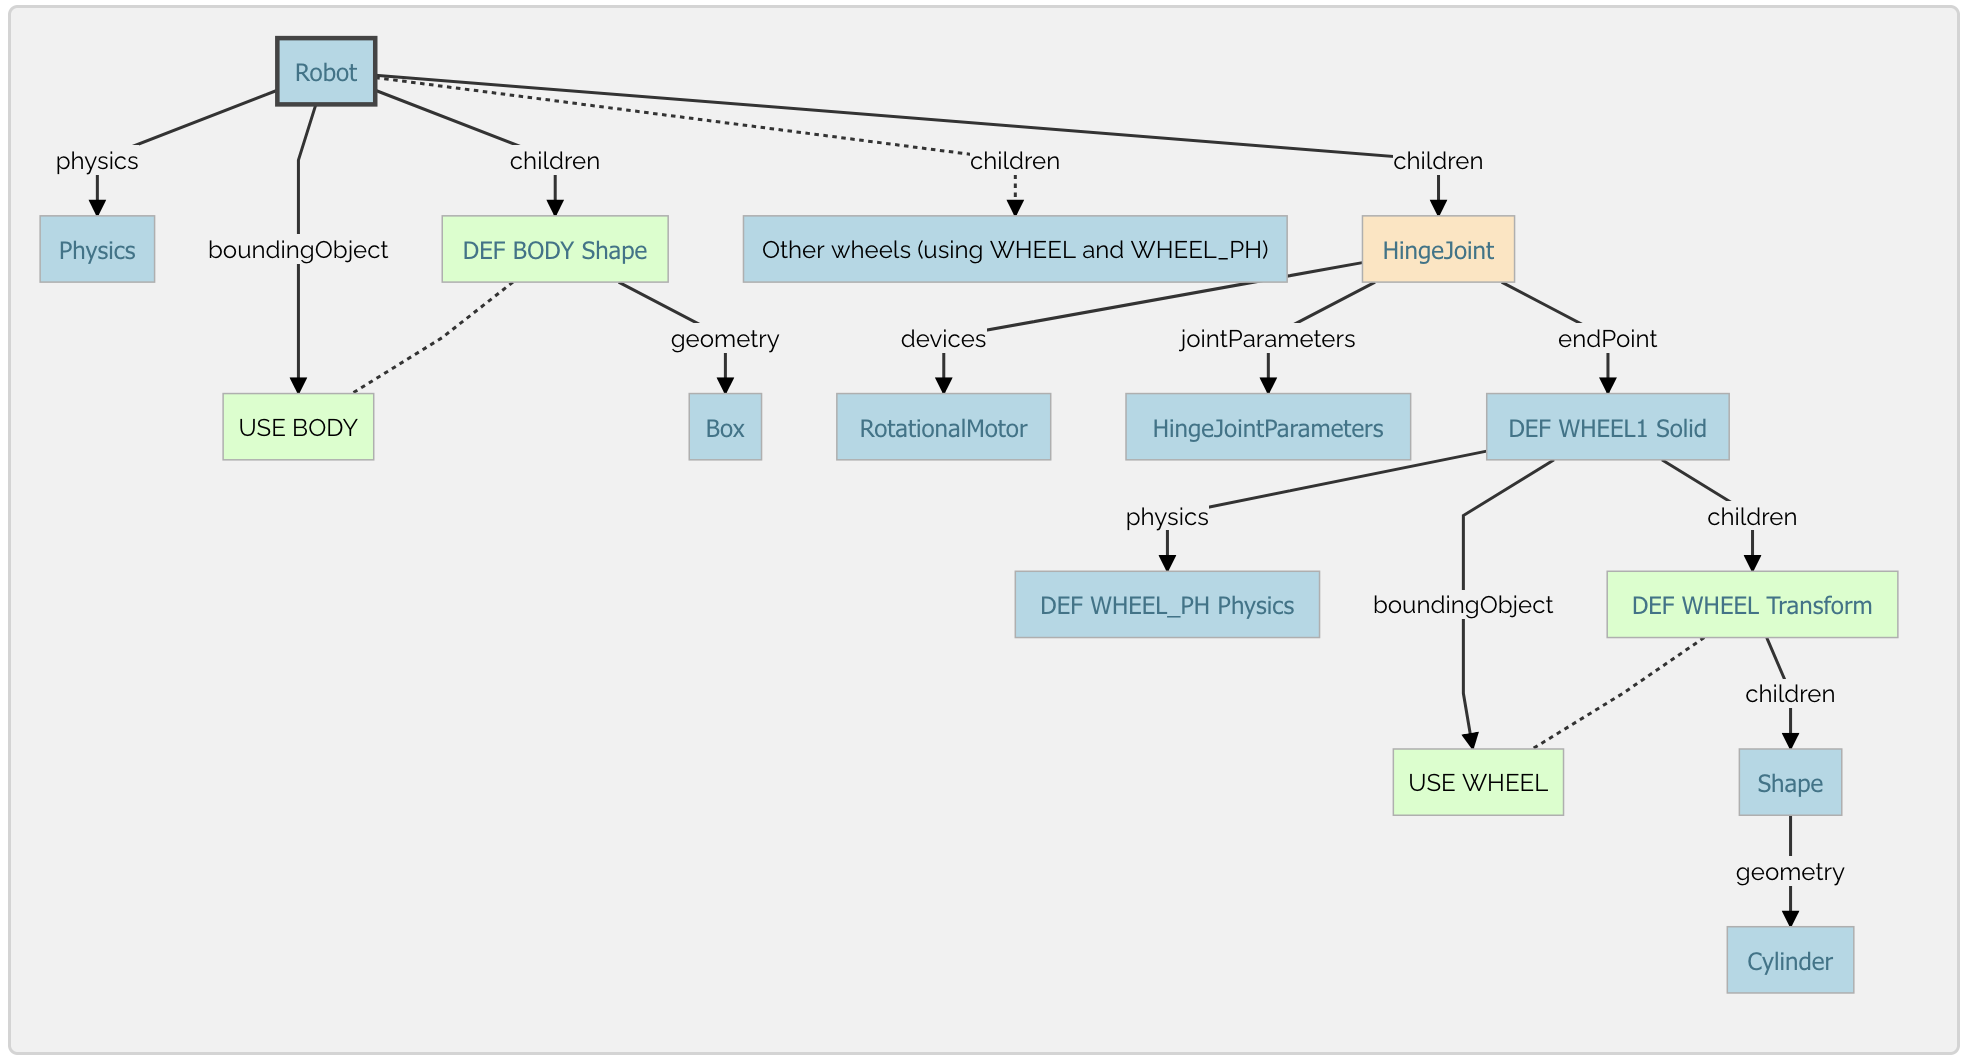
\includegraphics[width=0.99\columnwidth]{images/robot.png}
\end{columns}

\end{frame}

\begin{frame}[fragile]
\frametitle{Контроллер Webots}
\begin{itemize}
  \item Поле \cmd{controller} у робота задает управляющую программу, которая может обращаться к датчикам и управлять моторами
  \item Робот с правами \cmd{supervisor TRUE} может читать и изменять через контроллер состояние сцены и всех объектов в ней.
  \item В режиме \cmd{synchronization TRUE} симуляция приостанавливает расчет физического мира и ждет, пока код контроллера выполнит свой текущий шаг и вернет управление.
  \item Если задать \cmd{controller \textquotedbl\textless extern\textgreater\textquotedbl}, то управление будет передано внешней программе с передачей данных по IPC/TCP.
\end{itemize}

\small 
\end{frame}


\section{Webots и ROS2}

\begin{frame}
\frametitle{Связь Webots с ROS2}
\centering
\small
\vfill
\renewcommand{\arraystretch}{1.15}
\begin{tabular}{>{\raggedright\arraybackslash}m{0.27\textwidth}>{\raggedright\arraybackslash}m{0.64\textwidth}}
\toprule
\textcolor{HSEblue}{Участник} & \textcolor{HSEblue}{Роль} \\
\midrule
Webots & Симуляция \\
WebotsLauncher & Организует запуск симулятора и открывает нужную сцену \\
WebotsController & Контроллер робота, который передает данные между ROS2 и Webots \\
Узлы ROS2 & Читают данные датчиков, выполняют алгоритмы, публикуют команды. \\
\bottomrule
\end{tabular}\\[10pt]
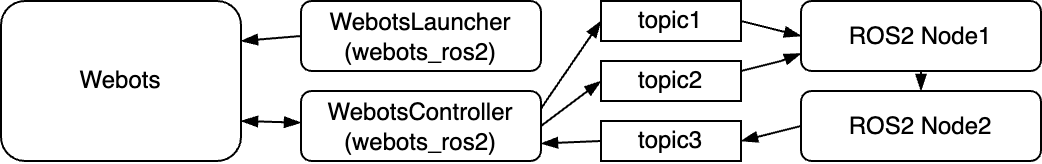
\includegraphics[width=0.85\columnwidth]{images/webots_ros2.png}
\end{frame}


\begin{frame}[fragile]
\begin{center}
\Large Спасибо за внимание!
\end{center}
\vfill
\end{frame}

\end{document}
